\documentclass{article}

% Import packages
\usepackage{graphicx}
\usepackage{float}
\usepackage{hyperref}

\usepackage{embedfile}
\usepackage{hypgotoe}

% Import code packages
\usepackage{listings}
\usepackage{color}

\definecolor{dkgreen}{rgb}{0,0.6,0}
\definecolor{gray}{rgb}{0.5,0.5,0.5}
\definecolor{mauve}{rgb}{0.58,0,0.82}

\lstset{frame=tb,
  language=Python,
  aboveskip=3mm,
  belowskip=3mm,
  showstringspaces=false,
  columns=flexible,
  basicstyle={\small\ttfamily},
  numbers=none,
  numberstyle=\tiny\color{gray},
  keywordstyle=\color{blue},
  commentstyle=\color{dkgreen},
  stringstyle=\color{mauve},
  breaklines=true,
  breakatwhitespace=true,
  tabsize=3
}

% Create custom environments

% \begin{reusefigure}[<float spec>]{<ref>}
% From https://tex.stackexchange.com/questions/225052/using-a-figure-again-in-document
\newenvironment{reusefigure}[2][htbp]
  {\addtocounter{figure}{-1}%
   \renewcommand{\theHfigure}{dupe-fig}% If you're using hyperref
   \renewcommand{\thefigure}{\ref{#2}}% Figure counter is \ref
   \renewcommand{\addcontentsline}[3]{}% Avoid placing figure in LoF
   \begin{figure}[#1]}
  {\end{figure}}

% Embed files
\embedfile{../data/alaska crime rates.csv}

% Document setup
\setlength{\parindent}{0pt}
\setlength{\parskip}{1em}
\title{Workshop 3: Maths, Graphs, and All Things Holy}
\author{Hatless Studios}
\date{\today}

\begin{document}
    \maketitle
    
    \section{Getting to your first graph}
    Today you were (probably) introduced to vectors and matrices for the first time. They're really simple structures that are \bfseries really \mdseries powerful.
    
    Despite this intuitive example on the board:

    \begin{figure}[H]
        \begin{center}
            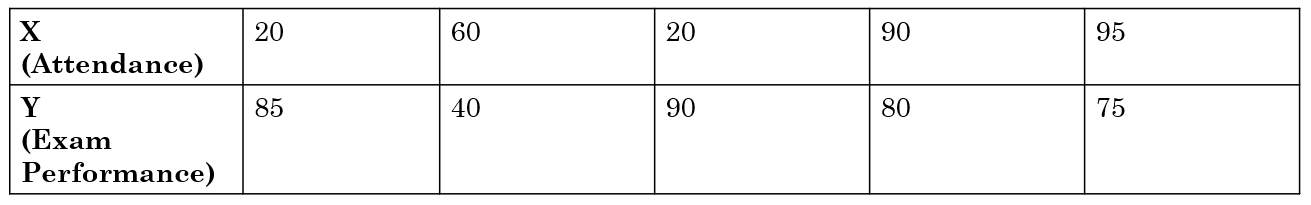
\includegraphics[width=\textwidth]{../figures/attendance-example}
            \caption{A matrix of attendance and exam performance.}
        \end{center}
        \label{fig:attendance}
    \end{figure}
    
    You still probably don't know how to actually create this in Python yet. What's particularly sneaky about matrices is that these are technically just \bfseries two lists \mdseries arranged in a fancy way that makes them easier to use...
    
    What if we could make use of this secret?!

    \subsection{Get your matrices over here!}
    You should be able to create matrices by using a nifty function called "np.array()". Here's an example usage... but it is not the answer to the attendance matrix!
    
    (See the next page for the example.)
    \newpage
    \begin{lstlisting}
        # This is done as a convention! 'np' is just easier to refer to then 'numpy' all the time.
        import numpy as np
        
        # Note here that I use 'one' and 'three'. Your variables in Python can't start with a number, such as '1'.
        one_dimensional_matrix = np.array([1, 5, 9])
        print(one_dimensional_matrix)
        
        one_dimensional_matrix = one_dimensional_matrix * 3
        print(one_dimensional_matrix)
        
        # Three Dimensional Time
        three_dimensional_matrix = np.array([[1, 0, 0], [0, 1, 0], [0, 0, 1]])
        print(three_dimensional_matrix)
        
        three_dimensional_matrix = three_dimensional_matrix * 2
        print(three_dimensional_matrix)
        
        print("===")
        print("ME CHANGING THE NUMBER 1")
        print("===")
        three_dimensional_matrix[0][1] = 1
        print(three_dimensional_matrix)
        
        print("===")
        print("EASIER WAY")
        print("===")
        an_easier_way = np.array([(1, 0, 0), (0, 1, 0), (0, 0, 1)])
        print(an_easier_way)
    \end{lstlisting}

    OUTPUT:
    \begin{lstlisting}
        [1 5 9]
        [ 3 15 27]
        [[1 0 0]
         [0 1 0]
         [0 0 1]]
        [[2 0 0]
         [0 2 0]
         [0 0 2]]
        ===
        ME CHANGING THE NUMBER 1
        ===
        [[2 1 0]
         [0 2 0]
         [0 0 2]]
        ===
        EASIER WAY
        ===
        [[1 0 0]
         [0 1 0]
         [0 0 1]]
    \end{lstlisting}

    Note: If when you try to run this code you get the error "ModuleNotFoundError: No module named 'numpy'", go to Command Prompt (or Terminal if you're on Mac) and type in "pip install numpy". This will install the missing 'numpy' package to your computer. If you run into issues like this in the future, that's how you solve them!

    This is all the information you need to be able to represent attendance as a matrix.

    \subsection{Question 1: Into the Matrix}
    \begin{reusefigure}[H]{fig:attendance}
        \begin{center}
            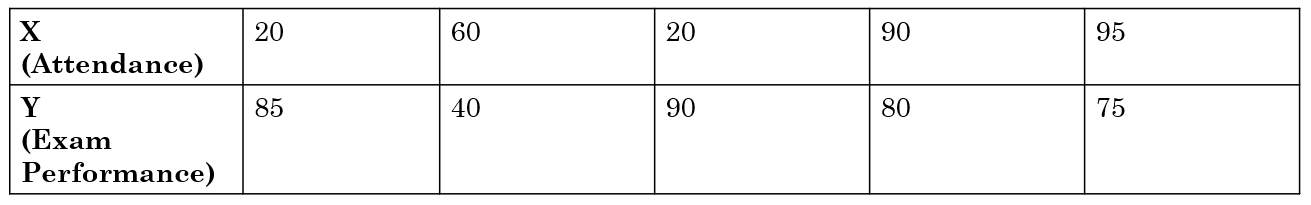
\includegraphics[width=\textwidth]{../figures/attendance-example}
            \caption{A matrix of attendance and exam performance.}
        \end{center}
    \end{reusefigure}

    Represent the attendance and exam performance table as a matrix in Python.

    \subsubsection{Helpful Resources}
    \bfseries What does np.array do? And what other things can I do that use this same 'ndarray' (n-dimensional array) data structure? \mdseries

    \url{https://numpy.org/doc/1.18/reference/generated/numpy.array.html}

    Alternatively, you can check the slides for more information. You would have been sent this in your email before the session.

    \subsection{Question 2: Literally Magic}
    In the slides there was an example function called 'f'.

    f(x) = 3x + 2

    Numpy has a really interesting feature that makes doing things to an entire matrix, no matter how many dimensions it has, really simple to do. This was covered in the presentation. One could say it was straight up bananas. Let's use that trick for ourselves.

    Apply the f function over your entire matrix.

    \section{Make your first graph!}
    Time to do something with that matrix you've got there.

    To quote the slides again, there was this pretty cool code that already graphs stuff. It will be easier to help you understand perhaps from there.

    \begin{figure}[H]
        \centering
        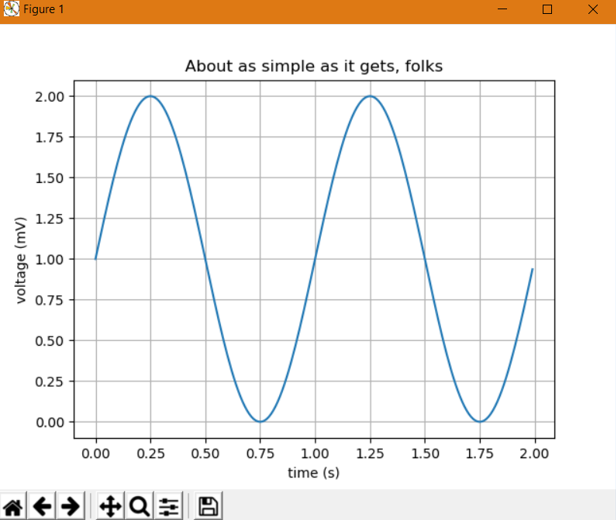
\includegraphics[width=\linewidth]{../figures/simple-graph.png}
        \caption{A simple line graph showing a mysterious device's voltage over time.}
        \label{simple-graph}
    \end{figure}

    \begin{lstlisting}
        import matplotlib
        import matplotlib.pyplot as plt
        import numpy as np
        
        t = np.arange(0.0, 2.0, 0.01)
        s = 1 + np.sin(2 * np.pi * t)
        
        fig, ax = plt.subplots()
        ax.plot(t, s)
        
        ax.set(xlabel='time (s)', ylabel='voltage (mV)',
            title='About as simple as it gets, folks')
        ax.grid()
        
        fig.savefig("ok.png")
        plt.show()
    \end{lstlisting}

    This code is all you need to plot your first graph. Read into the code and play around with it. Remember: decompose the problem into steps if it's got you confused. You can do this. I believe in you. What does each 'section' of code do? What is each line trying to achieve? How might you change what it does?

    \subsection{Question 3: This Is What You Came For}
    Plot the attendance matrix as a graph.

    \subsection{Question 4: Why's My Graph Broke?}
    When you've done this, you might notice your graph looks extremely weird. It's because matplotlib doesn't know what \bfseries range \mdseries you're graph is supposed to plot from, so it just checks the data for its answer. Use ax.set\_ylim() and its accompanying lim function for the 'x' of the graph to fix this.

    Check the resources below to help you with how to use it, and where that accompanying function might be.

    \subsubsection{Helpful Resources}
    \bfseries How do I do things with the 'ax' variable? \mdseries

    The 'ax' variable's data type (Remember integers and floats? Those are both data types, and are both types of numbers. This is the same thing. It's just 'ax' isn't a number, it's its own data type.) is called 'Axes'. Find out more about how to use this data type to your advantage here:

    \url{https://matplotlib.org/api/axes_api.html#matplotlib.axes.Axes}

    \bfseries How can I tinker around more with my graph? \mdseries
    
    The matplotlib documentation page that talks about the plot() function can give you the answers you desire:

    \url{https://matplotlib.org/api/_as_gen/matplotlib.pyplot.plot.html}

    \bfseries How do I change the type of graph? \mdseries
    
    This matplotlib doc page that talks about how to use the ax variable (from previous examples, which is one of the results returned from plt.subplots()) can tell you ALL kinds of ways you can plot two matrices of data (look for the 'Plotting' heading):
    
    \url{https://matplotlib.org/api/axes_api.html#matplotlib.axes.Axes}

    If you want \bfseries actual \mdseries code and graph examples, check out this page:

    \url{https://matplotlib.org/gallery/index.html}

    \section{Let's Get Real}
    In life you're not going to be given a matrix with 2 dimensions and 5 columns to be plotted. Usually, it's 2 dimensions and about 100 columns (as each column represents a record of data). And even more oftenly, \bfseries they're not even matrices. \mdseries

    It's time to get real and start dealing with actual files. Let's combine the things we've learned from past lessons!

    \subsection{Come one, come all - grab your data!}
    On my search for creating this workshop, I realized that data is literally just lying out there on the web, ready for some pesky students such as you and I to start just plotting random cheesecake from it. How convenient!

    \url{http://www.statpoint.net/OpenSample.aspx}

    However for the sake of simplicitly, and so we actually have an answers sheet for the other teachers to help you with code problems, and because it's actually a giant pain to get data from that website, I've taken the liberty of preparing some "interesting enough" (real) data for you to plot. Don't feel limited though. If you feel adventurous, go for it. We should still be able to help.

    \subsection{Question 5: Crime Over Time}
    When you downloaded this pdf file, along with it, there was an \texttt{alaska crime rates.csv} file. Yep, you guessed it, you're going to be using Alaska's crime rates.

    In the previous workshop, you learned how to open a file and put data into a list. Perhaps if you did the \bfseries extra spicy challenges \mdseries that were sent about a week ago, you'd have streamed the contents of 2 files into one dictionary. Fancy.

    Use everything you've learnt so far to plot a line graph of Alaska's total crime rate over the years.

    Remember, check the Helpful Resources above if you need a pick me up.

    \subsection{Question 6: Comparison Is the Thief of Joy}
    Time to take things up a notch.

    Along with the pdf file you also have an \texttt{alabama crime rates.csv} file. Sounds like it's time to compare two states.

    Plot a line graph comparing the total crime rates of Alaska and Albama over the years.

    \subsection{Question 7: Where Are We Headed?}
    When you're not messing around with them in coding workshops, graphs are actually very useful for understanding the \bfseries relationship \mdseries between two things. For example, is the crime rate getting worse?

    To answer this question, draw the trend lines of both Alaska and Alabama.

    \section{The Third Dimension}
    \subsection{Question 8: Time to Make Odd Three-Dimensional Things}
    \begin{figure}[H]
        \centering
        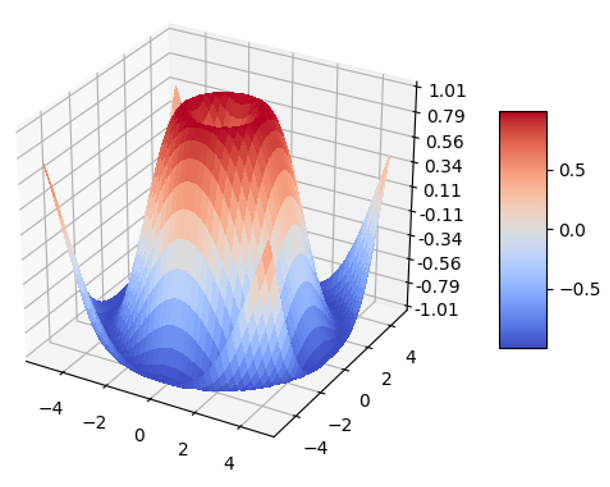
\includegraphics[width=\linewidth]{../figures/odd-3d-thing}
        \caption{An odd, three-dimensional \bfseries mesh graph \mdseries showing... something?}
        \label{odd-3d-graph}
    \end{figure}
    It wasn't fair of me to tease you with this during the presentation. After all of this effort you've gone through, it's finally time you faced the final boss. The three-dimensional beast.
    You might want the code for this... thing... as a reference point, so here you go:
    \newpage
    \begin{lstlisting}
        # This import registers the 3D projection, but is otherwise unused.
        from mpl_toolkits.mplot3d import Axes3D  # noqa: F401 unused import
        
        import matplotlib.pyplot as plt
        from matplotlib import cm
        from matplotlib.ticker import LinearLocator, FormatStrFormatter
        import numpy as np
        
        
        fig = plt.figure()
        ax = fig.gca(projection='3d')
        
        # Make data.
        X = np.arange(-5, 5, 0.25)
        Y = np.arange(-5, 5, 0.25)
        X, Y = np.meshgrid(X, Y)
        R = np.sqrt(X**2 + Y**2)
        Z = np.sin(R)
        
        # Plot the surface.
        surf = ax.plot_surface(X, Y, Z, cmap=cm.coolwarm,
                               linewidth=0, antialiased=False)
        
        # Customize the z axis.
        ax.set_zlim(-1.01, 1.01)
        ax.zaxis.set_major_locator(LinearLocator(10))
        ax.zaxis.set_major_formatter(FormatStrFormatter('%.02f'))
        
        # Add a color bar which maps values to colors.
        fig.colorbar(surf, shrink=0.5, aspect=5)
        
        plt.show()        
    \end{lstlisting}
    As a future reference, if you hadn't gone to the link on a Helpful Resources section yet, you can find this graph and more at \url{https://matplotlib.org/gallery/index.html}.

    You might be wandering how this is going to be useful to us at all. Honestly, I was thinking the exact same thing. Then I realized something. Some truly beautiful things happen when you've got \bfseries two data sets \mdseries.

    Plot a three-dimensional graph (it could be a mesh graph as shown above or a three-dimensional line graph) comparing a year of the difference between Alaska and Alabama's total crime rate compared to every other year.

    Why is this useful? Because it looks AMAZING. And you also practically will have mastered Matplotlib by the end of this. Good luck! Make sure to refer back to previous Helpful Resources posts to assist with the question.
\end{document}